\documentclass{article}
\usepackage[utf8]{inputenc}
\usepackage{hyperref}
\usepackage{listings}
\usepackage{multimedia} % to embed movies in the PDF file
\usepackage{graphicx}
\usepackage{comment}
\usepackage[english]{babel}
\usepackage{amsmath}
\usepackage{amsfonts}
\usepackage{wrapfig}
\usepackage{multirow}
\usepackage{verbatim}
\usepackage{float}
\usepackage{cancel}
\usepackage{caption}
\usepackage{subcaption}
\usepackage{mathdots}
\usepackage{/home/cade/Homework/latex-defs}


\title{MATH 582G Homework 5}
\author{Cade Ballew \#2120804}
\date{February 24, 2023}

\begin{document}
	
\maketitle
	
\section{Problem 1}
Consider the sets
\begin{align*}
&\real^n_{++}=\{x\in\real^n:x_i>0,i=1,\ldots,n\},\\
&\mathcal{S}^n_{++}=\{X\in\mathcal S^n:X\succ0\},
\end{align*}
and functions $f:\real^n_{++}\to\real$, $F:\mathcal{S}^n_{++}\to\real$ with
\[
f(x)=-\sum_{i=1}^n\log x_i,\quad F(X)=-\log\det X.
\]
\subsection{Part 1}
We have that
\[
\frac{\partial f(x)}{\partial x_i}=-\frac{1}{x_i},
\]
so 
\[
\nabla f(x)=\begin{pmatrix}
	-1/x_1\\
	\vdots\\
	-1/x_n
\end{pmatrix}.
\]
Then, 
\[
\nabla^2f(x)=\begin{pmatrix}
	1/x_1^2\\
	&\ddots\\
	&&1/x_n^2
\end{pmatrix}.
\]
\subsection{Part 2}
We have that 
\begin{align*}
F(X+tV)-F(X)&=-\log\det(X+tV)+\log\det(X)\\&=-\log\left(\frac{\det(X+tV)}{\det(X^{1/2})\det(X^{1/2})}\right)\\&=
-\log\left(\det(X^{-1/2})\det(X+tV)\det(X^{-1/2})\right)\\&=
-\log\det\left(X^{-1/2}(X+tV)X^{-1/2}\right)\\&=-\log\det\left(I+tX^{-1/2}VX^{-1/2}\right).
\end{align*}
Also, the cyclic invariance of the trace gives
\begin{align*}
t\langle X^{-1},V\rangle=t\tr(X^{-1}V)=t\tr(X^{-1/2}X^{-1/2}V)=t\tr(X^{-1/2}VX^{-1/2}).
\end{align*}
Thus,
\[
F(X+tV)-F(X)+t\langle X^{-1},V\rangle=-\log\det\left(I+tX^{-1/2}VX^{-1/2}\right)+t\tr(X^{-1/2}VX^{-1/2}).
\]
Letting $\mu_j$ denote the eigenvalues of $I+tX^{-1/2}VX^{-1/2}$, 
\begin{align*}
&-\log\det\left(I+tX^{-1/2}VX^{-1/2}\right)+t\tr(X^{-1/2}VX^{-1/2})\\&=-\log\prod_i(1+t\mu_i)+t\sum_i\mu_i=
\sum_i(-\log(1+t\mu_i)+t\mu_i)\\&=
\sum_i(-(\log(1)+t\mu_i+\oo(t))+t\mu_i)=\oo(t),
\end{align*}
where we have Taylor expanded the logarithm around 1. Thus,
\[
\lim_{t\to0}\frac{F(X+tV)-F(X)}{t}=-\langle X^{-1},V\rangle+\oo(1),
\]
so $\nabla F(x)=-X^{-1}$ by the definition of the gradient.

To compute the Hessian, we first observe that 
\[
(X+V)^{-1}=X^{-1/2}\left(I+X^{-1/2}VX^{-1/2}\right)^{-1}X^{-1/2}.
\]
Applying a Neumann series expansion,
\begin{align*}
(X+V)^{-1}&=X^{-1/2}\left(I-X^{-1/2}VX^{-1/2}+\OO(\|X^{-1/2}VX^{-1/2}\|^2_{\text{op}})\right)^{-1}X^{-1/2}\\&=X^{-1}-X^{-1}VX^{-1},
\end{align*}
if we drop higher order terms. Then
\begin{align*}
\lim_{t\to0}\frac{\nabla F(X+tV)-\nabla F(x)}{t}&=\frac{-(X+tV)^{-1}+X^{-1}}{t}\\&=\frac{-X^{-1}+tX^{-1}VX^{-1}+X^{-1}}{t}=X^{-1}VX^{-1}.
\end{align*}
Thus, $\nabla^2 F(X)[V]=X^{-1}VX^{-1}$.

\subsection{Part 3}
By the cylic invariance of the trace,
\begin{align*}
\langle\nabla^2 F(X)[V],V\rangle&=\tr(X^{-1}VX^{-1}V)=\tr(X^{-1/2}X^{-1/2}VX^{-1/2}X^{-1/2}V)\\&=
\tr\left((X^{-1/2}VX^{-1/2})(X^{-1/2}VX^{-1/2})\right)\\&=
\|X^{-1/2}VX^{-1/2}\|_F^2,
\end{align*}
which works if $X\succ0$ (allowing us to take the square root) and $V\in\mathcal S^n$. Since this is a norm, we must have that $\langle\nabla^2 F(X)[V],V\rangle>0$ when $V\neq0$, so $\nabla^2 F(X)$ is positive definite, and $F$ is convex.

\section{Problem 2}
We observe the following plots from applying GD and AGD to this function with an initial guess drawn from $N(0,I)$.
\begin{figure}[H]
	\centering
	\begin{subfigure}{0.495\linewidth}
		\centering
		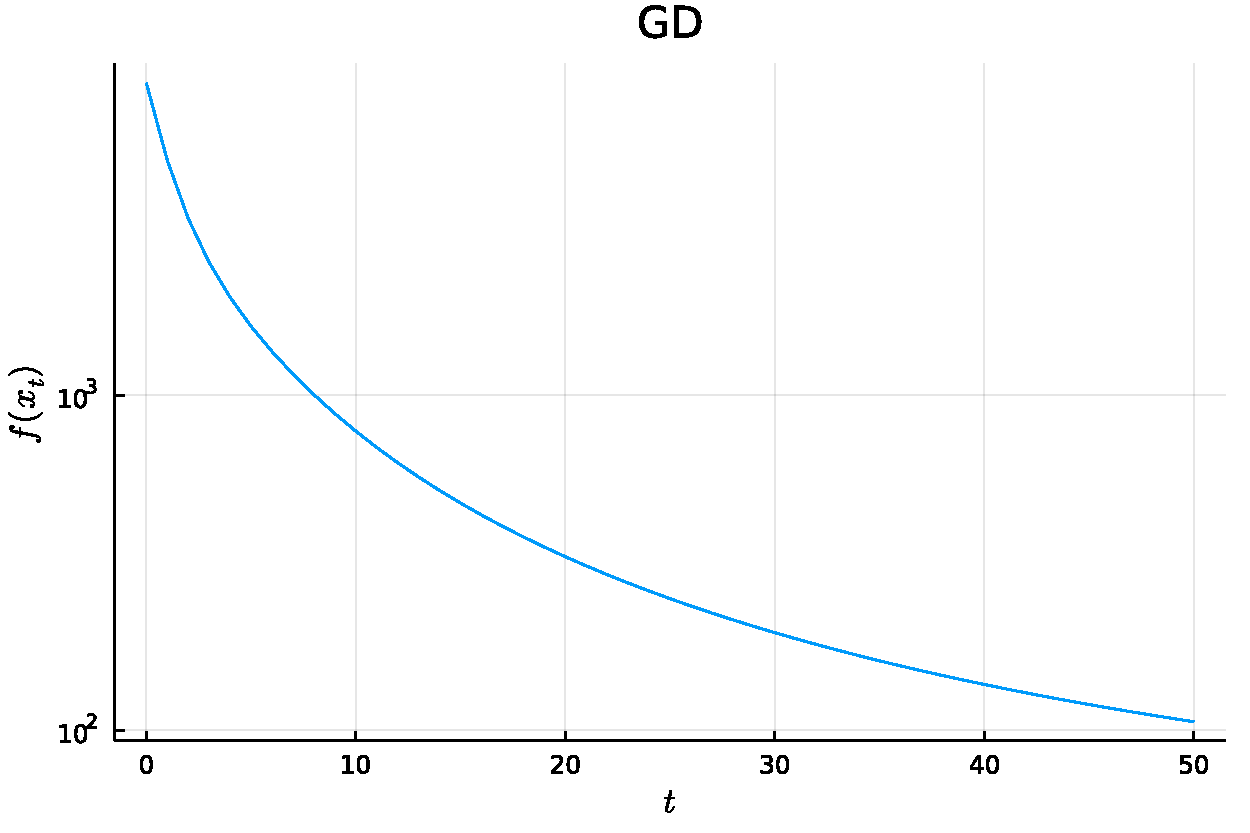
\includegraphics[width=\linewidth]{prob2a.pdf}
	\end{subfigure}
	\begin{subfigure}{0.495\linewidth}
		\centering
		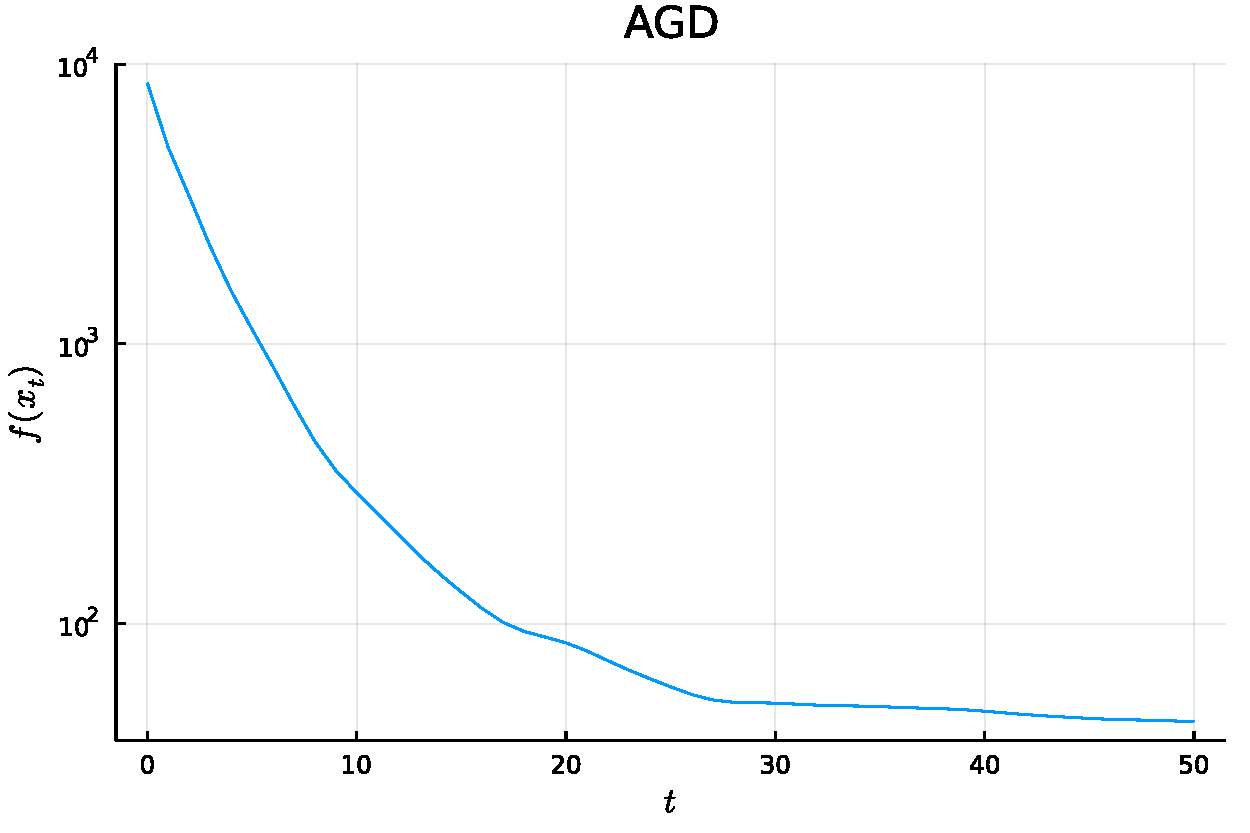
\includegraphics[width=\linewidth]{prob2b.pdf}
	\end{subfigure}
\end{figure}

\section{Problem 3}
We observe the following plots from applying GD and AGD to this function with an initial guess drawn from $N(0,I)$, $\eta=5$, and a stepsize of $2m\eta+\lambda$.
\begin{figure}[H]
	\centering
	\begin{subfigure}{0.495\linewidth}
		\centering
		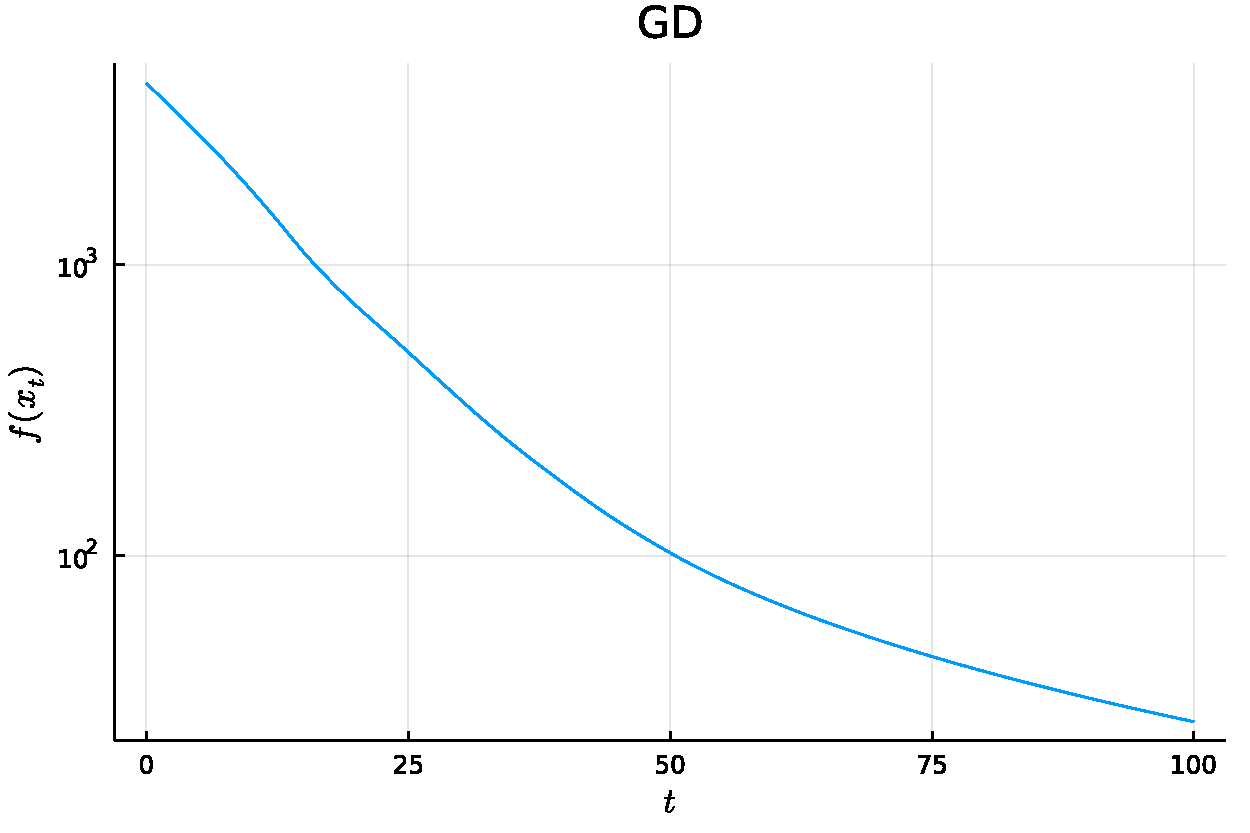
\includegraphics[width=\linewidth]{prob3a.pdf}
	\end{subfigure}
	\begin{subfigure}{0.495\linewidth}
		\centering
		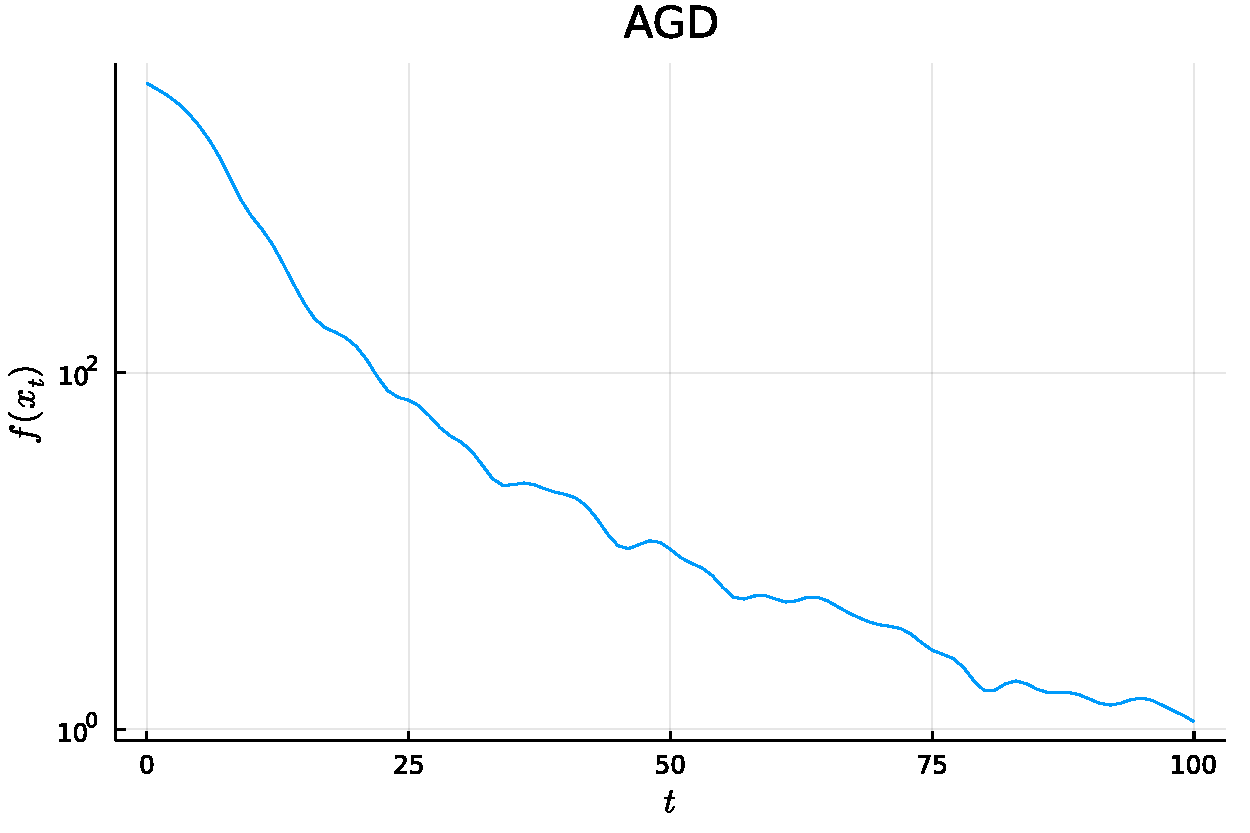
\includegraphics[width=\linewidth]{prob3b.pdf}
	\end{subfigure}
\end{figure}

\section{Problem 4}
We observe the following plots from applying GD and AGD to this function.
\begin{figure}[H]
	\centering
	\begin{subfigure}{0.495\linewidth}
		\centering
		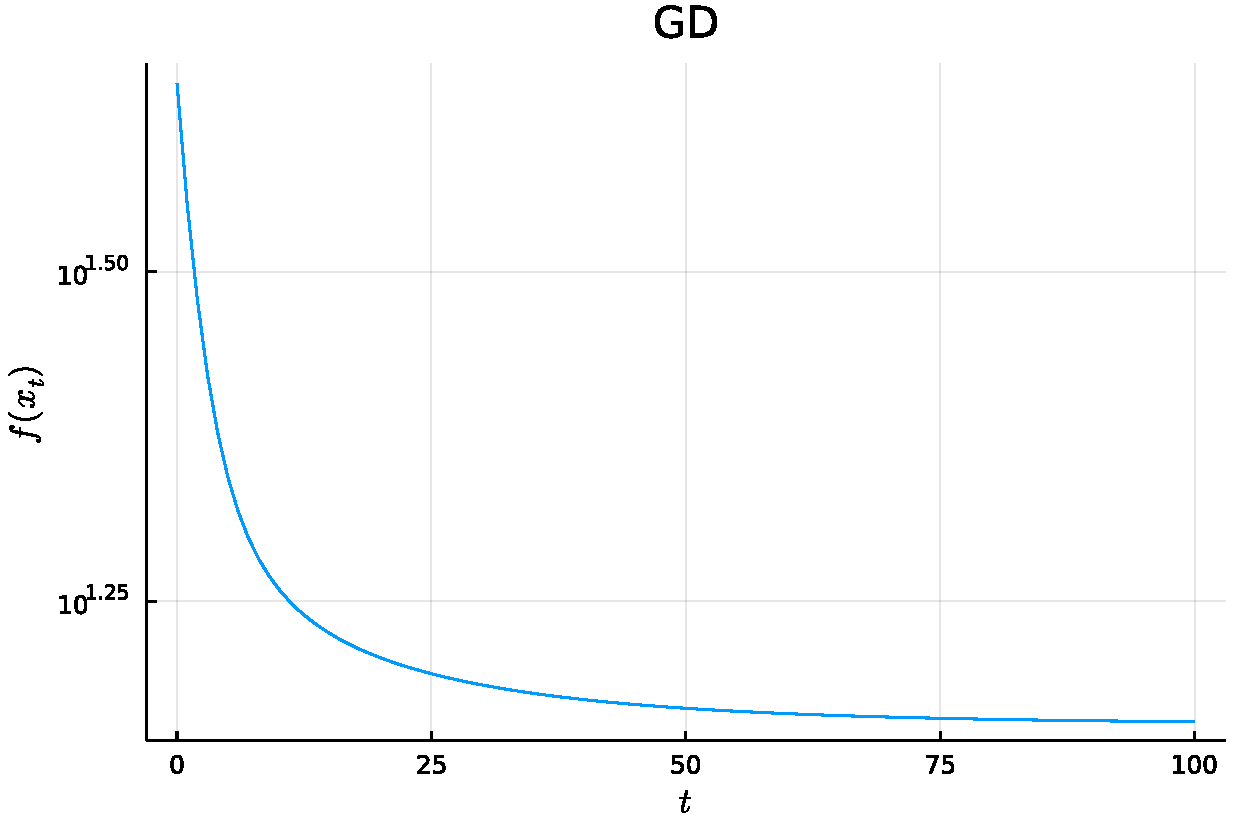
\includegraphics[width=\linewidth]{prob4a.pdf}
	\end{subfigure}
	\begin{subfigure}{0.495\linewidth}
		\centering
		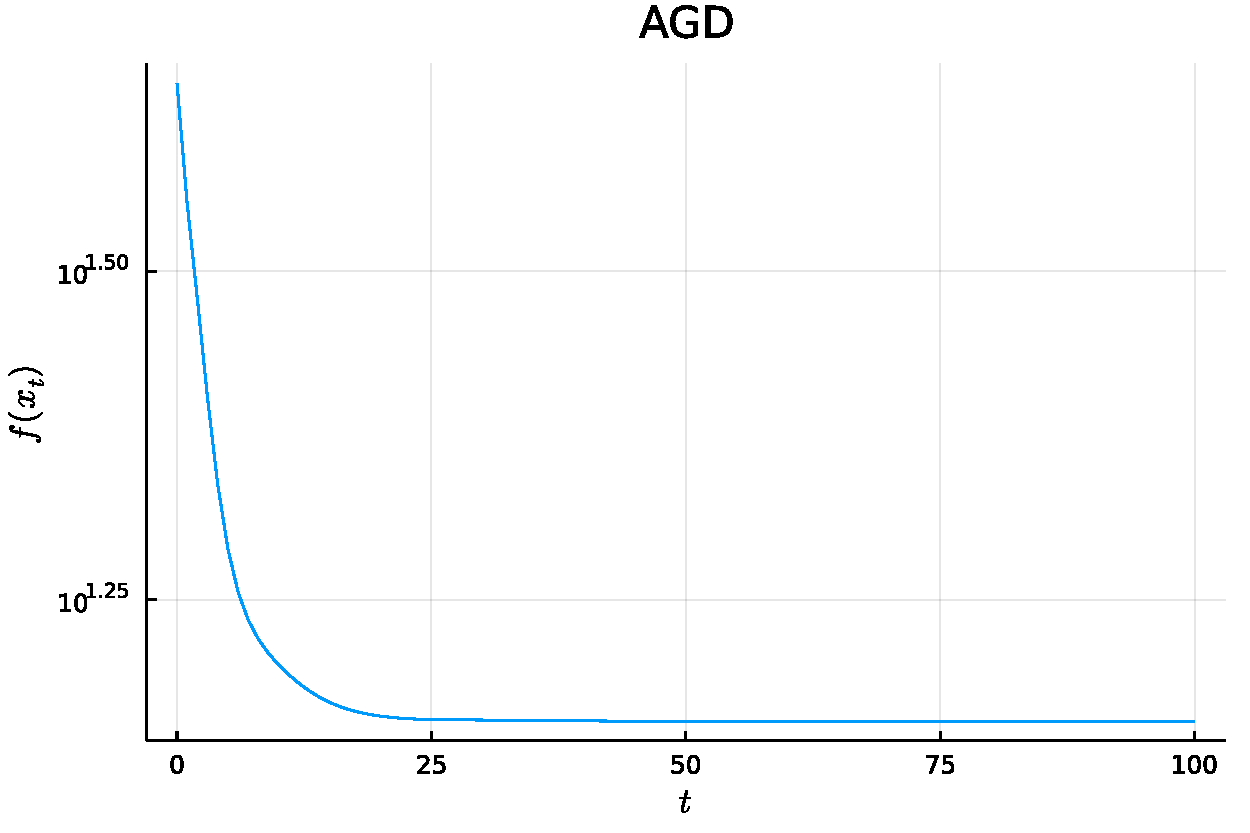
\includegraphics[width=\linewidth]{prob4b.pdf}
	\end{subfigure}
\end{figure}

\section{Problem 5}
Let $f:\real^d\to\real$ be a differentiable convex function and let $x^*$ be a minimizer. Consider the gradient descent iterates 
\[
x_{k+1}=x_k-\gamma_k\nabla f(x_k),
\]
for some sequence $\gamma_k\geq0$.
\subsection{Part 1}
We have that 
\begin{align*}
\frac{1}{2}\|x_{k+1}-x^*\|^2=\frac{1}{2}\|x_k-x^*\|^2+\langle x_{k}-x^*,x_{k+1}-x_k\rangle+\frac{1}{2}\|x_{k+1}-x_k\|^2.
\end{align*}
Clearly,
\[
\|x_{k+1}-x_k\|^2=\gamma_k^2\|\nabla f(x_k)\|^2.
\]
By convexity, we have that 
\begin{align*}
\langle x_{k}-x^*,x_{k+1}-x_k\rangle=-\gamma_k\langle x_{k}-x^*,\nabla f(x_k)\rangle\leq-\gamma_k(f(x_k)-f(x^*)),
\end{align*}
so
\[
\frac{1}{2}\|x_{k+1}-x^*\|^2\leq\frac{1}{2}\|x_k-x^*\|^2-\gamma_k(f(x_k)-f(x^*))+\frac{\gamma_k^2}{2}\|\nabla f(x_k)\|^2.
\]
\subsection{Part 2}
Suppose that the minimum of $f$ is given by $f^*$. Then, the RHS of the inequality from part 1 can be minimized by differentiating with respect to $\gamma_k$ and setting it equal to zero since it is convex in $\gamma_k$. This gives that 
\[
\gamma_k=\frac{f(x_k)-f^*}{\|\nabla f(x_k)\|^2}.
\]
Plugging this in to the inequality and scaling by 2, we have that 
\begin{align*}
\|x_{k+1}-x^*\|^2&\leq\|x_{k}-x^*\|^2-2\frac{f(x_k)-f^*}{\|\nabla f(x_k)\|^2}(f(x_k)-f^*)+\left(\frac{f(x_k)-f^*}{\|\nabla f(x_k)\|^2}\right)^2\|\nabla f(x_k)\|^2\\&\leq
\|x_{k}-x^*\|^2-\left(\frac{f(x_k)-f^*}{\|\nabla f(x_k)\|}\right)^2.
\end{align*}

\subsection{Part 3}
Also assume that $f$ is $\beta$-smooth.
%\begin{align*}
%\|x_{k+1}-x^*\|^2&\leq\|x_{k}-x^*\|^2-\left(\frac{f(x_k)-f(x^*)}{\|\nabla f(x_k)-\nabla f(x^*)\|}\right)^2\\&\leq
%\|x_{k}-x^*\|^2-\left(\frac{f(x_k)-f(x^*)}{\beta\|x_k-x^*\|}\right)^2
%\end{align*}
We can rearrange and write the telescoping sum
\begin{align*}
\sum_{i=0}^{k-1}\left(\frac{f(x_i)-f^*}{\|\nabla f(x_i)\|}\right)^2&\leq\sum_{i=0}^{k-1}\left(\|x_{i}-x^*\|^2-\|x_{i+1}-x^*\|^2\right)\\&=
\|x_{0}-x^*\|^2-\|x_{k}-x^*\|^2\leq\|x_{0}-x^*\|^2.
\end{align*}
Letting $j\in\{0,\ldots,k-1\}$ be the index for which $\|\nabla f(x_k)\|$ is maximized,
\begin{align*}
&\frac{1}{\beta\|x_0-x^*\|^2}\sum_{i=0}^{k-1}\left(f(x_i)-f^*\right)^2\leq\frac{1}{\beta\|x_j-x^*\|^2}\sum_{i=0}^{k-1}\left(f(x_i)-f^*\right)^2\\&\leq\frac{1}{\|\nabla f(x_j)\|^2}\sum_{i=0}^{k-1}\left(f(x_i)-f^*\right)^2\leq\sum_{i=0}^{k-1}\left(\frac{f(x_i)-f^*}{\|\nabla f(x_i)\|}\right)^2,
\end{align*}
by the definition of $\beta$-smoothness and the fact that $\nabla f(x^*)=0$. By Cauchy-Schwartz, we have that 
\[
\left(\sum_{i=0}^{k-1}\left(f(x_i)-f^*\right)\right)^2\leq k\sum_{i=0}^{k-1}\left(f(x_i)-f^*\right)^2,
\] 
so combining these,
\[
\left(\sum_{i=0}^{k-1}\left(f(x_i)-f^*\right)\right)^2\leq\beta^2k\|x_0-x^*\|^4.
\]
Now, we just take the square root, divide by $k$, and apply Jensen's inequality on the LHS to get that
\[
f\left(\frac{1}{k}\sum_{i=0}^{k-1}x_i\right)-f^*\leq\frac{\beta\|x_0-x^*\|^2}{\sqrt{k}}.
\]
If we additionally have that $f$ is $\alpha$-strongly convex, we begin with our original inequality and apply $\alpha$-convexity in the numerator and $\beta$-smoothness in the denominator to get that 
\begin{align*}
\|x_{k+1}-x^*\|^2\leq\|x_k-x^*\|^2-\left(\frac{\alpha\|x_k-x^*\|^2/2}{\beta\|x_k-x^*\|}\right)^2=\left(1-\frac{\alpha^2}{4\beta^2}\right)\|x_k-x^*\|^2.
\end{align*}

\end{document}
